\chapter{Evaluation Strategy for Taggle}
\label{chap:eval}
\ifpdf
    \graphicspath{{Chapters/Evaluation/EvaluationFigs/PNG/}{Chapters/Evaluation/EvaluationFigs/PDF/}{Chapters/Evaluation/EvaluationFigs/}}
\else
    \graphicspath{{Chapters/Evaluation/EvaluationFigs/EPS/}{Chapters/Evaluation/EvaluationFigs/}}
\fi  


Our systematic mapping study of tag cloud research (presented in Chapter~\ref{chap:strateval}) identified tag cloud visualisation as a technique had not been as extensively evaluated as other topics (such as interactive interfaces incorporating tag clouds), indicating opportunities for measuring effectiveness and developing ways to improve the tag cloud approach. No research identified in the mapping study described a system with interactive features like Taggle, where data fields from a multi-variate dataset are mapped to tag cloud visual properties. There were a limited range of evaluation approaches despite the widespread presence of interactive interfaces, typically utilising user performance measurements (\emph{visualisation use} type techniques), rather than strategies considering the \emph{data analysis process}, which are of high practical value and relevance when evaluating systems to explore data and discover information. We were therefore encouraged in several aspects: by focusing on software engineering we were promoting use of tag cloud visualisation outside the typical web and user generated data domains; that our tool was unique in its approach, and that to conduct an evaluation with broad-ranging goals we should consider multiple targeted evaluation strategies. 

Based on the results of the systematic study, this chapter outlines the process and outcomes of designing an evaluation plan for Taggle. We describe mapping out our overall evaluation strategy and associated methodologies in \S\ref{sect:evalstrat}, and evaluations that were selected to be conducted in \S\ref{sect:evals}. Generation of suitable datasets for experimentation is discussed in \S\ref{sect:dataselection}. In \S\ref{sect:eyetracker} we describe the process we took to conduct three of our experiments on an eye-tracking machine. 

%Two types of evaluation strategy (visualisation use and data analysis process) were introduced from the categories outlined by \citet{lam12} along with their relative goals, methodologies and pros/cons. 
%To evaluate Taggle in a balanced and broad manner, we split evaluations into two parts; one part to evaluate considerations with tag cloud visualisation itself (`visualisation use' category type), and one part that evaluated Taggle itself (`data analysis process' category type). The goal of the whole-system evaluation was to find out if and how Taggle supported user comprehension and exploration of relevant knowledge in the software engineering domain.

\section{Overall evaluation strategy}\label{sect:evalstrat}

Our overall goal for evaluation was to explore the potentials and limitations of our tag cloud visualisation tool Taggle. We decided to map out sample areas of the tool which were of interest, in order to strategically plan a broad-ranging series of evaluations. This map is represented in Figure~\vref{fig:evaluationmap}. Potential areas of evaluation were divided into the part of the system being looked at --- \emph{visual encoding} or \emph{interactive tool}. Each potential research question was associated with an appropriate evaluation strategy (highlighted in blue): \emph{User Performance, User Experience, Visual Data Analysis and Reasoning} (for more details of strategies identified by \citet{lam12} see Chapter~\ref{chap:strateval}). For each design choice or evaluation strategy, sample methodologies are outlined (presented in a white cloud).

\begin{landscape} %make this single page display as landscape
\begin{figure}[!htb]
   	\centering
  	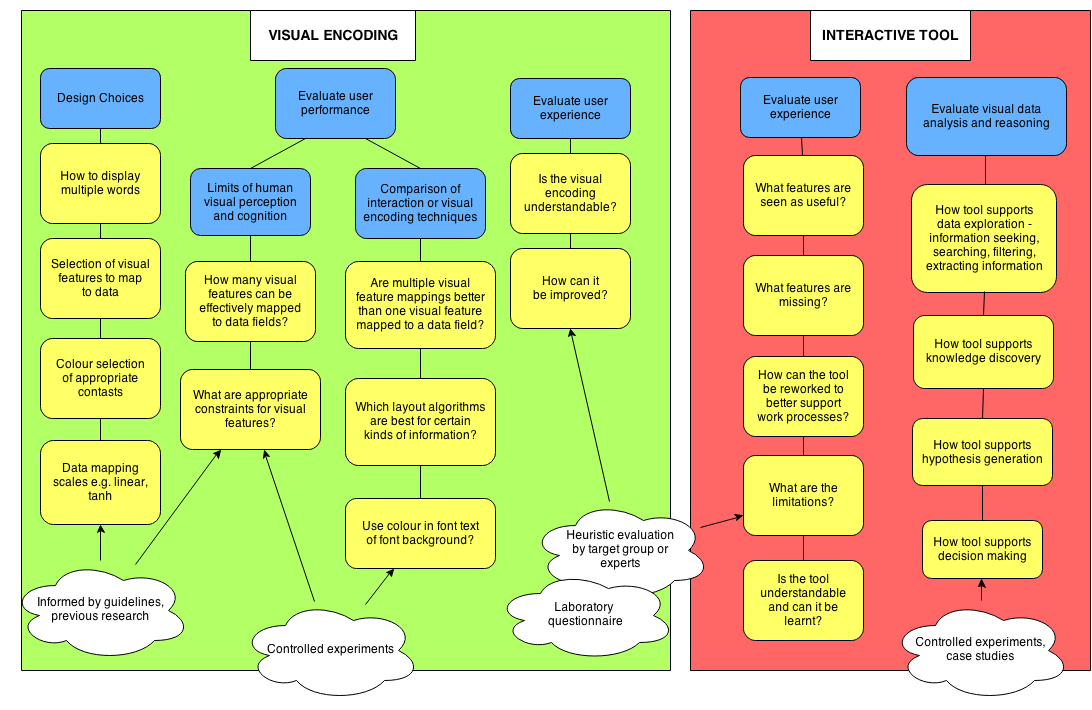
\includegraphics[scale=0.6]{TaggleEvaluation.png}	
	\caption{\textit{Evaluation strategy map for an interactive tag cloud visualisation tool}}
	\label{fig:evaluationmap}
\end{figure}
\end{landscape}

In the green box on the map under the \emph{visual encoding} section, there are a list of \emph{design choices} that needed to be made. Selection of approaches could be made either through controlled experiments comparing choices, or relevant information found in previously defined guidelines, research or design principles. Questions regarding the visual encoding of the tool that are suited to evaluation by \emph{user performance} are divided into understanding the limits of human visual perception and cognition, or involving a comparison of interaction or visual encoding techniques. These questions can be answered by experimentation if no previous research exists. Additionally, visual encoding of the tool may benefit from evaluation of \emph{user experience}, where questions are answered through subjective user questionnaires or the process of heuristic evaluation.

In the red box section describing research questions for the \emph{interactive tool}, there is a second set of \emph{user experience} questions which may be answered by heuristic evaluation or laboratory questionnaire. An evaluate \emph{visual data analysis and reasoning} section defines research questions related to decision making and knowledge discovery, where responses can be gathered from case studies or user experiments with the interactive tool.

Ultimately, the creation of this map was a highly worthwhile experience as it allowed us to select the most appropriate evaluation methodologies for the research questions in which we were interested. 

\section{Selected evaluations}\label{sect:evals}

Many of the design choices that were possible for the visual encoding of the tool had been made according to the design considerations outlined in Chapter~\ref{chap:tagcloud} which were informed by guidelines or other research. A decision was made to conduct user experiments comparing the enhanced tag cloud features which were included in Taggle with tag clouds generated in a more conventional fashion. Two experiments were designed for the following special features:

\begin{itemize}
\item the use of background colour to increase the colour space of the tag text
\item the use of multiple visual features to highlight and reinforce data mappings 
\end{itemize}

\paragraph{Use of background colour} Small tags in Taggle (or any tag cloud visualisation) are inevitable if we are using a full range of tag sizes. In software engineering we are dealing with lots of tags due to the large dataset sizes, and we need to know if users can identify the variables mapped to colour, should they be displayed with smaller tags (or Taggle's small iconified tags). Use of background colour --- which increases the amount of colour space of the tag text --- may help here. 

\paragraph{Use of multiple visual mappings} We think mapping multiple visual features may be helpful for users to identify data correlations, through highlighting and reinforcing selected data mappings. Reinforcing these all important mappings may also assist users to explore the data more effectively. 

\paragraph{}These experiments are a good starting point in our evaluation plan, laying the foundations for more specific targeting of other areas of Taggle's visual encoding in future. Two different layouts were also tested in each experiment. The experiments compared user visual search response times (a \emph{user performance} evaluation strategy) and were conducted on an eye-tracking machine. Details can be found in Chapters~\ref{chap:exp1} and \ref{chap:exp2}.

An evaluation with domain experts using a special heuristic set for information visualisation was planned to elicit user experience feedback on both the visual encoding and interactive tool. Subjective user feedback was sought to clarify research questions regarding the comprehensibility of the visualisation technique, as well as assessing the system usability. Outcomes of this evaluation are discussed in Chapter~\ref{chap:heuristiceval}.

A \emph{visual data analysis and reasoning} experiment was conducted to try to discover if (and how) Taggle supports data exploration for a software engineering dataset. This was a whole-tool approach focused on the knowledge discovery process. Chapter~\ref{chap:exp3} details the executed experiment and results. 

\section{Dataset generation}\label{sect:dataselection}

Previous tag cloud research has used a variety of sources for experiments requiring tag corpora. In general, for quantitative experiments the tag labels themselves were taken from real life data such as psycholinguistic databases \citep{bateman08, rivadeneira07}, online sources such as Flickr, Zoomclouds \citep{schrammel09, kaser07} or contained encyclopaedic-type categorical data (unspecified sources) \citep{oosterman10, halvey07} while the tag weightings were generated artificially to match experiment goals. These experiments focused on datasets with a more conventional tag cloud application in mind (web site content visualisation for example), and were using only one weighting. Creation of tag corpora for a multi-variate dataset is a more complex affair as we are concerned with multiple variables. For realism in tasks both general and in the software engineering domain, we need the data to make sense, with variables containing correlations and realistic distributions. In addition, we need to avoid user bias which might occur in datasets where users could be expected to have some personal knowledge.

We required two types of datasets in our experiments. For the \emph{visualisation use} experiments (Chapters~\ref{chap:exp1} and \ref{chap:exp2}), we wanted to use datasets from a general domain (to widen both the pool of participants and potential datasets) containing categorical data with a nominal data field which could be used as a text label for tags. Like previous research, we chose to source the textual data fields from real life data and selected lesser-known knowledge areas to minimise bias. Data for numeric variables in the same dataset were generated artificially. For the second type of dataset for use in the \emph{data analysis process} evaluation, we required a software engineering dataset. This was generated in the same way as the general domain datasets, with class names taken from an open source project and software metrics generated artificially. See Figure~\vref{fig:datasets} for example datasets compiled from both real life data and generated data.

It also would have been possible in many cases to have used a subset of the original data rather than artificial generation, but this would have required careful analysis first to discover outliers/distributions and other special features. Taking a subset may have affected the dataset features in unintended ways whereas artificial data generation gave absolute control over the correlations and features of the dataset.

\begin{figure}[!htb]
\centering
\begin{subfigure}{.5\textwidth}
	\centering
	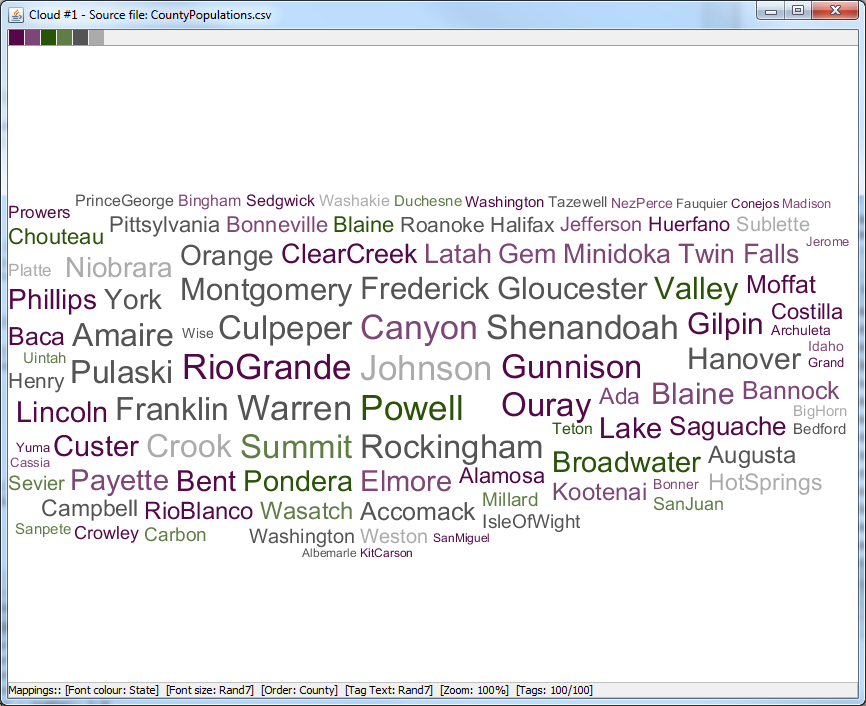
\includegraphics[scale=0.25]{C2S2L1.png}
	\caption{\textit{Populations of counties in the USA}}
\end{subfigure}%
\begin{subfigure}{.5\textwidth}
  \centering
  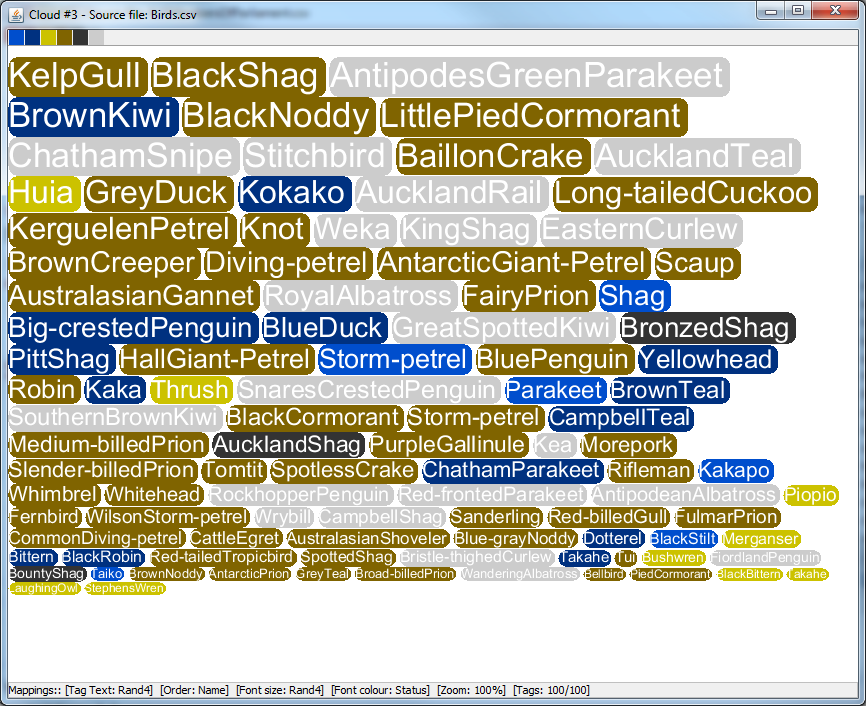
\includegraphics[scale=0.25]{C1S1L2.png}
  \caption{\textit{Extinction categories of birds in NZ}}
\end{subfigure}
\begin{subfigure}{.5\textwidth}
  \centering
  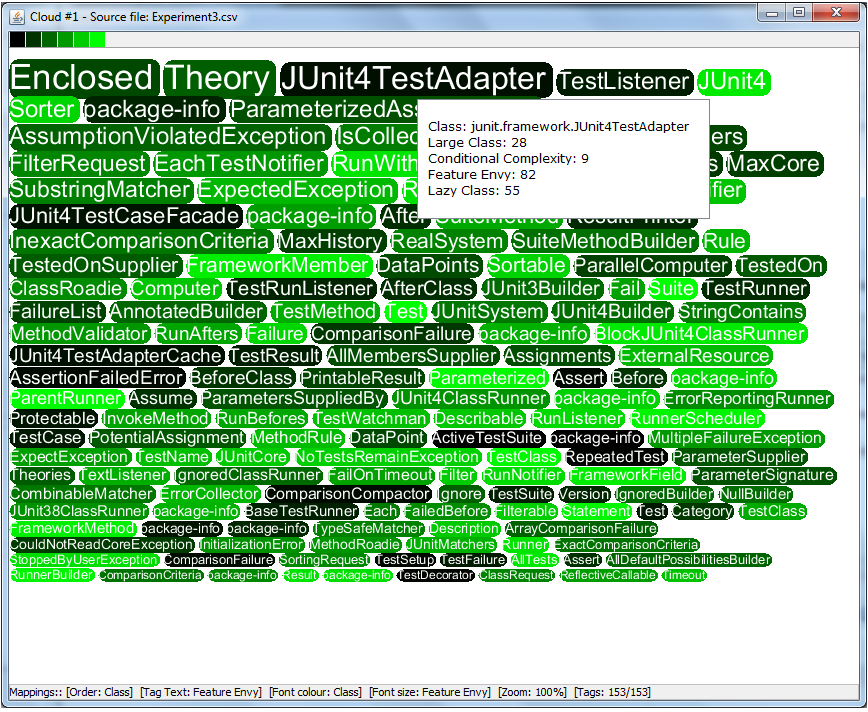
\includegraphics{exp3.png}
  \caption{\textit{Code smells in open source project JUnit}}
\end{subfigure}%
  \caption{\textit{Examples of datasets compiled from both real life and artificially generated data}}
  \label{fig:datasets}
\end{figure}

\section{Conducting an eye-tracking experiment}\label{sect:eyetracker}

Experiments in Chapters~\ref{chap:exp1}, \ref{chap:exp2} and \ref{chap:exp3} were performed using an eye-tracking machine. Eye-tracking is the technique used to capture and measure eye movements, allowing analysis to be performed on the patterns of visual attention of a user performing a series of specific tasks. From these analyses, inferences can be made about the user's cognitive processes \citep{olsen10}. Eye-movement is typically divided into two types 1) saccades (quick movements of the eye from one location to another) and 2) fixations (cessation of the eye movement, pausing on an object of interest for a period of time). Eye-tracking data is collected and then interpreted through visual representations such as gaze plots (a presentation of saccades between fixations, showing the eye scan path), or heat maps showing time spent at each fixation (example Figure~\vref{fig:visualfeaturesearch} for an example of a gaze plot).

Experiments were performed using a Tobii T60 eye-tracker. This has an optimal operating distance of 65 cm, so the participant must be place approximately this far away from the eye-tracker. The T60 can capture stimuli at a maximum radius of 35 degrees and is integrated with a high resolution 17'' monitor. 

Figure~\vref{fig:eyetrackpipeline} shows the pipeline process which was followed using the Tobii studio software to complete experiment design and recording through to statistical data exportation. Tobii studio was used to input the experimental design with selected test media and manage the participants and experiment counter-balancing. During the experiment process, participant eye-movement was recorded. Areas of interest (target tags) were defined within the tag cloud images and the software collected metrics regarding those areas of interest (such as the time to first fixation). The software was used to play back video recordings with eye-movements, to manually analyse eye movement search patterns within the media.

\begin{figure}[!htb]
   	\centering
  	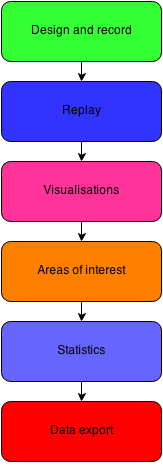
\includegraphics[scale=0.60]{pipeline.png}	
	\caption{\textit{Pipeline of an eye-tracking experiment}}
	\label{fig:eyetrackpipeline}
\end{figure}

\section{Summary and discussion}

Our systematic mapping study of tag cloud research showed us that to broadly evaluate Taggle we should consider multiple targeted evaluation strategies. To that end, we followed a procedure of mapping out our overall evaluation strategy based on evaluation approaches presented by \citet{lam12}. From this map we selected evaluations and appropriate methodologies. Experimentation conducted from this map required generation of realistic datasets sourced from both general and software engineering domains. Three of our experiments were run on eye-tracking machines, allowing us to perform analysis on patterns of user visual attention. The process of conducting an eye-tracking experiment also required carefully management and adherence to a pipeline process from experiment design to statistical data exportation. 

% ------------------------------------------------------------------------


%%% Local Variables: 
%%% mode: latex
%%% TeX-master: "../thesis"
%%% End: 
